\subsection{Wind Turbine}

The 400 watt Sunforce wind turbine was mounted atop the Fish building, URI bay campus. The ground elevation is 60 feet about the North American Datum of 1983. The location has high ground to the west as well as an adjacent building. Although this is less than ideal, it will be nearly impossible to mount the package in a location where the bridge will not block wind from one or many directions.  A 60 watt light bulb was used as a load for the system. 

\indent The turbine is very responsive to changes in wind direction and is susceptible to becoming unstable during gusts. For this reason the voltage from the turbine can be seen dramatically spiking during times of the day, figure \ref{fig:wind}. On 02 May 2014, starting at 08:24:32 PM the turbine went for over 16 hours with zero energy produced. 

\begin{figure}
\centering
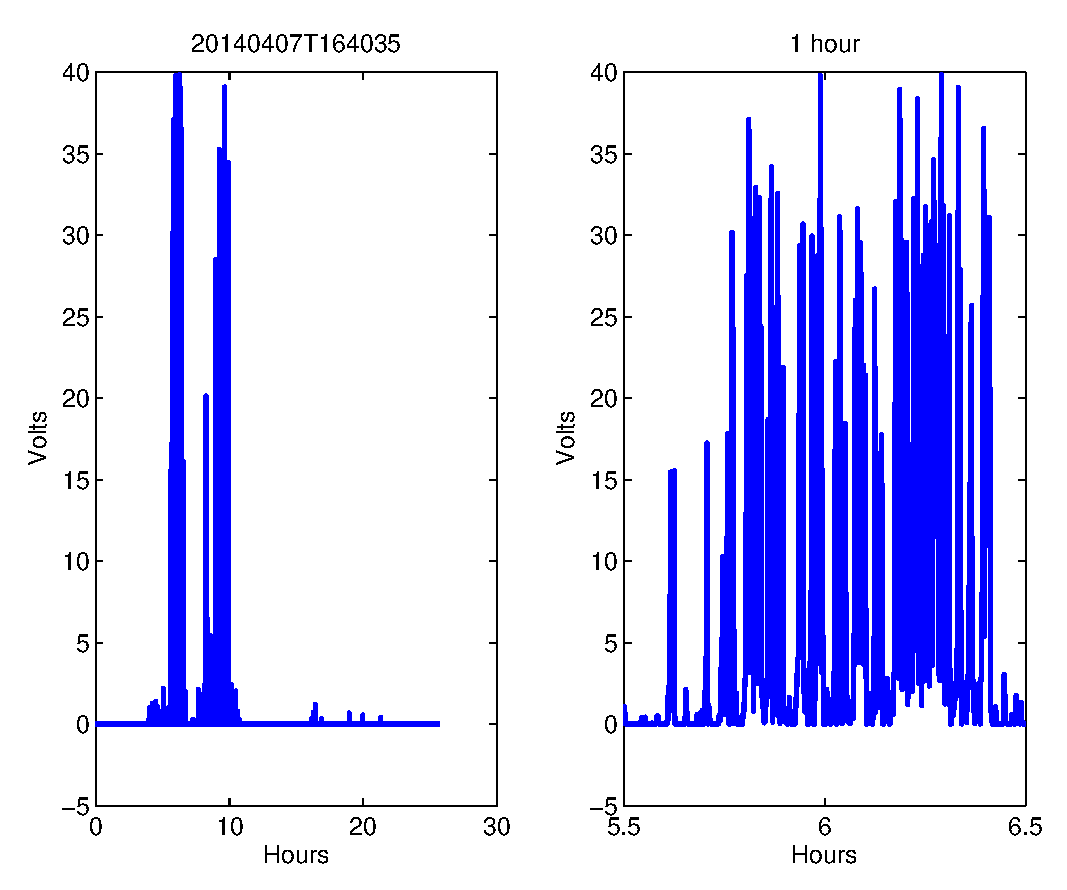
\includegraphics[width = \textwidth]{WESLEY_wind.eps}
\caption{\textit{Voltage output from turbine}}
\label{fig:wind}
\end{figure}